\section{Master-Theorem}

\begin{frame}{Teile und herrsche -- divide and conquer}
	\begin{itemize}
		\item Probleminstanz in kleinere Teile zerlegen
		\item Teile rekursiv nach gleichen Verfahren bearbeiten
		\item Aus Teilergebnissen Resultat rekonstruieren
	\end{itemize}
\end{frame}

\begin{frame}{Das Master-Theorem (einfache Form)}
	Situation aus dem Leben: 
	\begin{itemize}[<+->]
		\item Wir haben einen rekursiven Algorithmus $A(n)$ für die Problemgröße $n$
		\item Bei jedem Schritt wird das Problem um $b$ geteilt und es ergeben sich $a$ neue Probleminstanzen der Größe $n/b$
		\item Wie können die Laufzeit der jeweiligen \enquote{Auseinandernehmungs-} und \enquote{Zusammenführungsschritte} \textbf{linear} abschätzen.
	\end{itemize}
\end{frame}

\begin{frame}{Das Master-Theorem (einfache Form)}
	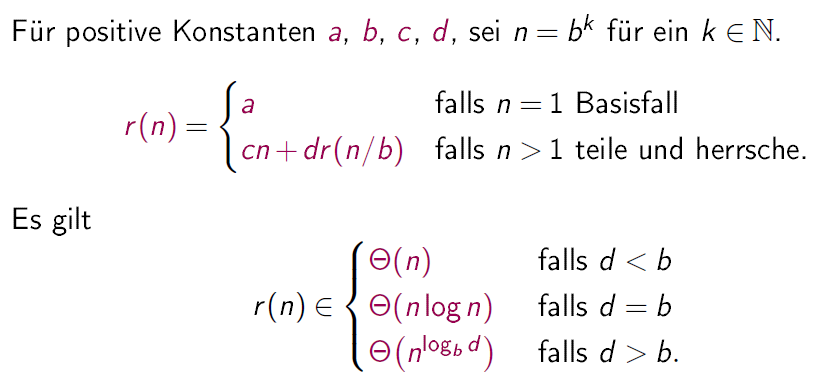
\includegraphics[scale=0.5]{laufzeit/masterTheorem}
\end{frame}

\begin{frame}{MT: Beispiele}
	Wir betrachten verschiedene Sortierverfahren:\\
	\bigskip
	
	\textbf{Mergesort}\\
	msort(L: Liste mit |L| = n):\\
		teile L in der Mitte auf in $L_1$ und $L_2$\\
		sortiere $L_1$ und $L_2$\\
		füge $L_1$ und $L_2$ in O($n$) zusammen\\
	\medskip
	
	$$r(n) = \pause \begin{cases}
	1 & n = 1\\
	c \cdot n + 2 \cdot r(n/2) & n > 1
	\end{cases}$$
	
	\pause
	Nach MT, Fall 2 also: $r(n) \in \Th{n \log n}$
\end{frame}

\begin{frame}{MT: Beispiele}
	Wir betrachten verschiedene Sortierverfahren:\\
	\bigskip
	
	\textbf{DoubleMergesort}\\
	dmsort(L: Liste mit |L| = n):\\
	teile L in der Mitte auf in $L_1$ und $L_2$\\
	sortiere $L_1$ und $L_2$ \textbf{jeweils zwei mal}\\
	\textit{Ja, das hat natürlich keinerlei Sinn und ist rein konstruiert}\\
	füge $L_1$ und $L_2$ in O($n$) zusammen\\
	\medskip
	
	$$r(n) = \pause \begin{cases}
	1 & n = 1\\
	c \cdot n + 4 \cdot r(n/2) & n > 1
	\end{cases}$$
	
	\pause
	Nach MT, Fall 3 also: $r(n) \in \Th{n^2}$
\end{frame}

\begin{frame}{MT: Beispiele}
	Wir betrachten verschiedene Sortierverfahren:\\
	\bigskip
	
	\textbf{Magicsort}\\
	msort(L: Liste mit |L| = n):\\
	teile L in der Mitte auf in $L_1$ und $L_2$\\
	sortiere $L_1$\\
	$L_2$ ist an dieser Stelle durch Magie bereits sortiert\\
	füge $L_1$ und $L_2$ in O($n$) zusammen\\
	\medskip
	
	$$r(n) = \pause \begin{cases}
	1 & n = 1\\
	c \cdot n + 1 \cdot r(n/2) & n > 1
	\end{cases}$$
	
	\pause
	Nach MT, Fall 1 also: $r(n) \in \Th{n}$
	\medskip
	
	\textbf{ACHTUNG:} Magicsort kann es nicht geben! In Algorithmen I:\\ 
	Untere Schranke für vergleichsbasiertes Sortieren ist $\Om{n \log n}$
\end{frame}


\begin{frame}{Limitierungen des MT}
	Das Master-Theorem ist mächtig, aber leider längst nicht so mächtig, wie der Name es vielleicht vermuten lässt.\\
	\pause
	Dieses (einfache) MT funktioniert nur bei sehr speziellen Rekkurenzformen (auch wenn diese häufig vorkommen).\\
	\pause
	Ein erweitertes MT wurde in der VL vorgestellt, ist aber auch nicht vollständig!\\
	\pause
	\medskip
	Bei ungleichen Aufteilungen hilft einem das MT überhaupt nicht weiter:\\
	Berechnet man $(n + 1)! = n! \cdot (n + 1)$, so kann die Laufzeit der Berechnung nicht mit dem MT abgeschätzt werden.
\end{frame}